\usetikzlibrary{shapes.geometric, calc}

\begin{figure}[h]
\centering
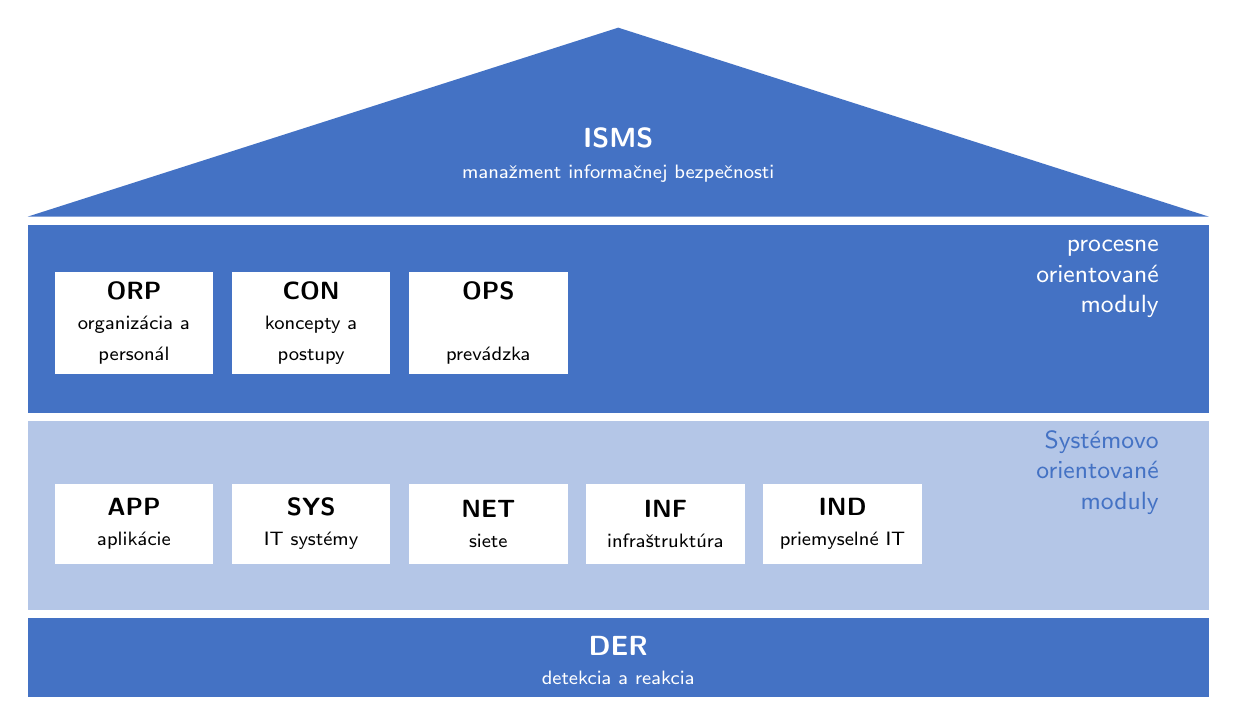
\begin{tikzpicture}[
    every node/.style={font=\sffamily},
    box/.style={
        rectangle,
        draw=white,
        fill=white,
        minimum width=2.0cm,
        minimum height=1.0cm,
        align=center,
        font=\sffamily\small
    }
]

\definecolor{midblue}{RGB}{68, 114, 196}
\definecolor{lightblue}{RGB}{180, 198, 231}

\fill[midblue] (0, 0) rectangle (15, 1.0);
\node[text=white, font=\sffamily\bfseries] at (7.5, 0.65) {DER};
\node[text=white, font=\sffamily\scriptsize] at (7.5, 0.25) {detekcia a reakcia};

\fill[lightblue] (0, 1.1) rectangle (15, 3.5);
\node[text=midblue, font=\sffamily\small, anchor=north east] at (14.7, 3.55)
    {\begin{tabular}{r}Systémovo\\orientované\\moduly\end{tabular}};
\node[box] at (1.35,  2.2) {\textbf{APP}\\\scriptsize aplikácie};
\node[box] at (3.6,   2.2) {\textbf{SYS}\\\scriptsize IT systémy};
\node[box] at (5.85,  2.2) {\textbf{NET}\\\scriptsize siete};
\node[box] at (8.1,   2.2) {\textbf{INF}\\\scriptsize infraštruktúra};
\node[box] at (10.35, 2.2) {\textbf{IND}\\\scriptsize priemyselné IT};

\fill[midblue] (0, 3.6) rectangle (15, 6.0);
\node[text=white, font=\sffamily\small, anchor=north east] at (14.7, 6.05)
    {\begin{tabular}{r}procesne\\orientované\\moduly\end{tabular}};
\node[box] at (1.35,  4.75) {\textbf{ORP}\\\scriptsize organizácia a \\\scriptsize personál};
\node[box] at (3.6, 4.75) {\textbf{CON}\\\scriptsize koncepty a\\\scriptsize postupy};
\node[box] at (5.85,  4.75) {\textbf{OPS}\\\\\scriptsize prevádzka};

\fill[midblue] (0, 6.1) -- (7.5, 8.5) -- (15, 6.1) -- cycle;
\node[text=white, font=\sffamily\bfseries] at (7.5, 7.1) {ISMS};
\node[text=white, font=\sffamily\scriptsize] at (7.5, 6.65) {manažment informačnej bezpečnosti};


\end{tikzpicture}
\caption{Vrstvový model, prevzatý z \cite{GSK} a upravený, tmavomodré pozadie sú procesné moduly a bledomodré pozadie sú systémove moduly.}
\label{fig:gsk-layer-model}
\end{figure}